\section{Experiments}
\label{sec:experiments}

%\subsection{Data}
%\label{sec:data}
%\vspace{-2mm}


We tested our approach in two different domains, open-domain and cellular biology. For consistency we use the same corpora as Jansen et al.~\shortcite{jansen14}, which are described briefly here. 

{\flushleft {\bf Yahoo! Answers (YA):}}  Ten thousand open-domain \emph{how} questions were randomly chosen from the Yahoo! Answers\footnote{\url{http://answers.yahoo.com}} community question answering corpus and divided: 50\% for training, 25\% for development, and 25\% for test.  Candidate answers for a given question are selected from the corresponding answers proposed by the community (each question has an average of 9 answers).

{\flushleft {\bf Biology QA (Bio):}} 183 \emph{how} and 193 \emph{why}  questions in the cellular biology domain were hand-crafted by a domain expert, and paired with gold answers in the Campbell's Biology textbook~\cite{Reece:2011}.  Each paragraph in the textbook was considered as a candidate answer.  As there were few questions, five fold cross-validation was used with three folds for training, one for development, and one for test.

%In both set-ups, candidate answers were assigned a candidate retrieval (CR) score based on the lexical similarity of the question to the candidate answer.~\footnote{In the Bio task, the CR also incorporated a similarity between the question and the section containing the candidate answer paragraph.}  That CR score served as both a strong baseline for the models (when used alone) as well as an additional feature to be used alongside the model features described in section \ref{sec:models}.
%\subsection{Sources for Alignment}
%\label{sources}

{\flushleft {\bf Alignment Corpora}}: To train the alignment models we generated alignment pairs from two different resources: Annotated Gigaword \cite{Napoles2012} for YA, and the textbook for Bio.  Each was discourse parsed with the RST discourse parser described in Section~\ref{sec:approach}, which is implemented in the FastNLPProcessor toolkit\footnote{\url{http://github.com/sistanlp/processors}}, using the MaltParser\footnote{\url{http://www.maltparser.org/}} for syntactic analysis.
% and reimplements the discourse model of Feng and Hirst~\shortcite{feng12}, using solely features extracted from dependency syntax.


%To explore the relationship between amount of available training data and performance, after each resource was discourse parsed it was divided into samples of exponentially increasing size.  For AGiga, there were 12 sizes ranging from one document to 10,000 and for the textbook, there were 10 sizes ranging from one subsection up to the entire book (2686 subsections).  Additionally, there were 10 samples for each size to reduce the margin of error. 
%condense this---
%To demonstrate the utility of our approach in generating surrogate training data for limited resource domains, we evaluated the performance of our models with incremental amounts of data.  
%{\flushleft {\bf Annotated gigaword \todo{CITE}(AGiga)}}: After discourse parsing AGiga in its entirety, we randomly selected 10 files.  From each we made 12 samples that exponentially increased in size, from 1 document up to 10,000.~\footnote{The larger samples contained the same documents as the smaller samples from the same file so as to represent consistently growing knowledge.}  
%{\flushleft {\bf Campbells}}:For Bio, Campbell's textbook was divided at the subsection level, discarding any subsection consisting of only a single sentence, for a total of 2686 subsections.  These subsections were shuffled to generate 10 random permutations and 10 samples exponentially increasing in number of subsections were made from each.  

\subsection{Results and Discussion}
\label{sec:results}

\begin{figure}[t!]
\begin{center}
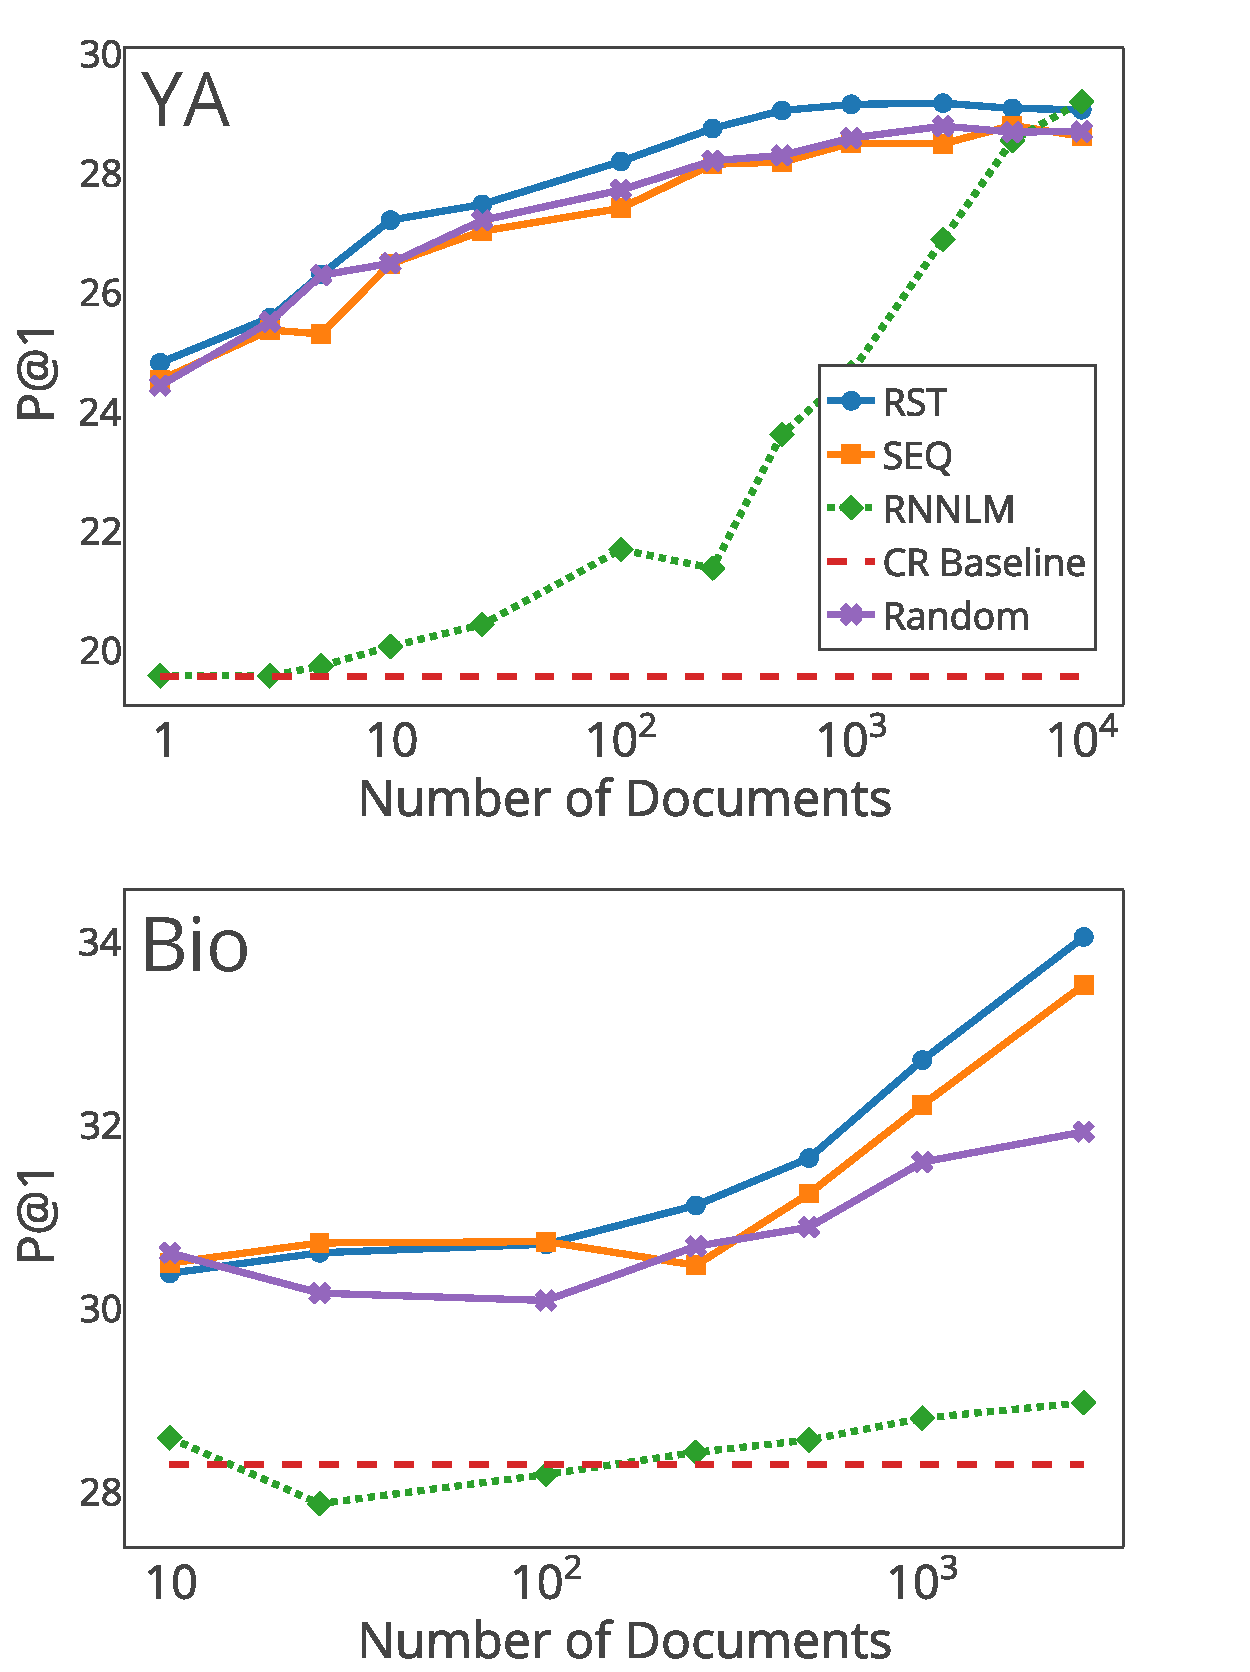
\includegraphics[width=75mm]{graphs_test2a.pdf}
%\vspace{-4mm}
\caption{{\small Overall performance for the two discourse-based alignment models,
compared against the CR baseline, random baselines, and a RNNLM-based reranker.
%, sequential, and lexical semantic models versus the number of training documents used to construct the models.  
The $x$ axis indicates the number of training documents used to construct all models. 
Each point represents the average of 10 samples of training documents.  }}
\vspace{-6mm}
\label{fig:performance}
\end{center}
\end{figure}

\begin{comment}
\begin{table}[t!]
\begin{center}
%\begin{scriptsize}
\begin{footnotesize}
\begin{tabular}{llc}
\multicolumn{1}{l}{ } & \multicolumn{1}{l}{ } & \multicolumn{1}{l}{P@1} \\
\multicolumn{1}{l}{ Model/Features } & \multicolumn{1}{l}{P@1} & \multicolumn{1}{l}{Impr.} \\
\cline{2-3}

\hline
\multicolumn{3}{l}{\textit{Yahoo! Answers}} \\ % 185q (sent) ret=1p c=0.1 
\hline
CR Baseline 	& 19.48 	&	  				\\
CR + RST  		& 28.98		& +48.75\% 			\\
CR + SEQ  		& 28.53		& +46.45\% 			\\
CR + RNNLM  		& 29.11		& +49.44\% 			\\
\hline
\multicolumn{3}{l}{\textit{Bio WHY}} \\ % 185q (sent) ret=1p c=0.1 
\hline
CR Baseline 	& 28.24 	&	  				\\
CR + RST  		& 34.00		& +20.38\% 			\\
CR + SEQ  		& 33.47		& +18.53\% 			\\
CR + RNNLM  		& 28.92		& +2.39\% 			\\
\end{tabular}
\end{footnotesize}
\caption{{\small Final performance for the discourse, sequential, and lexical semantic models as compared to the candidate retrieval baseline. For space reasons data for Bio WHY are shown but the pattern is essentially identical for Bio HOW.}}
\label{tab:overall}
\end{center}
\end{table}
\end{comment}
Figure \ref{fig:performance} shows the performance of the discourse models against the number of documents used to train the alignment model.\footnote{For space reasons the graph for Bio \emph{how} is not shown, but the pattern is essentially identical to Bio \emph{why}.}   We used the standard implementation for P@1 ~\cite{manning08} with the adaptations for Bio described in Jansen et al.~\shortcite{jansen14}. We address the following questions.
%, and compare against the CR baseline and RNNLM-based reranker.

\paragraph{How does the performance of the RST and SEQ models compare?}
% and to the baselines?}
Comparing the two principal alignment models, the RST-based model significantly outperforms the SEQ model by about 0.5\% P@1 in both domains (p $<$ 0.001 for Bio and p $<$ 0.01 for YA)\footnote{All reported statistics were performed at the endpoints, i.e., when all training data is used, using bootstrap resampling with 10,000 iterations.}. This shows that deep discourse analysis (as imperfect as it is today) is beneficial. 

\paragraph{How does the performance of the RST model compare to a model trained on in-domain pairs?}

Both the RST and SEQ results for YA are {\em higher} than that of an alignment model trained on explicit in-domain question-answer pairs. Fried et. al \shortcite{fried15} trained an identical alignment model using approximately 65k QA pairs from the YA corpus, and report a performance of 27.24\% P@1, or nearly 2 points lower than our model trained using 10,000 Gigaword documents. This is an encouraging result, which further demonstrates that: (a) discourse analysis can be exploited to generate artificial semi-structured data for alignment, and (b) the sequential model, which also outperforms Fried et. al, can be used as a reasonable proxy for discourse when a parser is not available. 


\paragraph{How does the performance of the RST model compare to previous work?}

Comparing our work to Jansen et al. \shortcite{jansen14}, the most relevant prior work, we notice two trends.
First, our discourse-based alignment models outperform their CR + RNNLM model, which peaks at 26.6\% P@1 for YA and 31.7\% for Bio \emph{why}. While some of this difference can be assigned to implementation differences (e.g., we consider only content words for both alignment and RNNLM, where they used all words), this result again emphasizes the value of our approach.
% Second, while our content-filtered RNNLM outperforms their unfiltered model\footnote{RNNLM performance is slightly less in Bio as we use only the textbook for training.}, when using equal amounts of training data, our alignment model trained using discourse still outperforms the RNNLM until the performance of all models ultimately plateaus in knowledge-rich environments.  
Second, the partially lexicalized discourse structures used by Jansen et. al to identify explanatory text in candidate answers perform better than our approach, which relies solely on lexicalized alignment. However, we expect that our two approaches are complementary, because they address different aspects of the QA task (structure vs. similarity).
%the performance of our alignment models be orthogonal to their discourse models, 
%as we don't explicitly use discourse structures to identify answer candidates in our reranker.

\paragraph{How do the RST and SEQ models compare to the non-alignment baselines?}

%Both the RST and SEQ alignment models \todo{significantly} %considerably 
%outperform the CR and RNNLM baselines, especially for few training documents or domain-specific (Bio) settings.\footnote{The immediate performance boost seen by the alignment models even for 1 training document is explained by the fact the the global alignment probability of Surdeanu et al. (2011) explicitly models word self associations, which complements well the vector space model of the CR baseline.}  

In Bio, both the RST and SEQ alignment models significantly outperform the RNNLM and CR baselines (p $<$ 0.001).  %Additionally, the RST model does significantly better than the SEQ model (p $<$ 0.001).  
In YA, the RST and SEQ models significantly outperform the CR baseline (p $<$ 0.001), and though 
%and the RST model also does significantly better than the RND baseline (p $<$ 0.05) though the SEQ does not (p $>$ 0.1).% as well as the SEQ model (p $<$ 0.01).  
they considerably outperform the the RNNLM baseline for most training document sizes, when all 10,000 documents are used for training, they do not perform  better.  
%Finally, the SEQ model is not significantly better than the RND baseline (p $>$ 0.1).
This shows that alignment models are more robust to little training data, but RNNLMs catch up when considerable data is available.

%RND??
%with both models approaching 34\% P@1 in Bio (or 20\% over the CR baseline), and 29\% P@1 in YA (up to a 49\% relative performance gain over the CR baseline). \textcolor{red}{In YA, when all training documents are used, the performance of the RST model was significantly higher the SEQ model (p $<$ 0.01) as well as all baselines (p $<$ *** for all).  The YA SEQ model performance was not significantly different than that of the RND baseline (p $>$ ***) but was ***.  In Bio...  As the amount of training data in Bio increases, performance gaps of the various models widen.  That is, when enough signal builds up, we can see the increase in efficacy of lexical associations when words go from simply being within the same domain (tRND), to broadly cohesive (SEQ), to finally having a fine-grained discourse connection (RST).}

\paragraph{How does the SEQ model compare to the RND baseline?}
In Bio, the SEQ model significantly outperforms the RND baseline (p $<$ 0.001) but in YA it does not.  This is likely due to differences in the size of the document which was randomized.  In YA, the sentences were randomized within Gigaword articles, which are relatively short (averaging 19 sentences), whereas in Bio the randomization was done at the textbook level.  In practice, as document size decreases, the RND model approaches the SEQ model.


%% Cut for space
%\paragraph{What is the contribution of the individual discourse relations used in generating the alignment pairs?}
%\begin{table}[t!]
%\begin{center}
%\begin{footnotesize}
%\begin{tabular}{llclc}
%\multicolumn{1}{l}{ } & \multicolumn{1}{c}{YA} & \multicolumn{1}{c}{Bio} 		\\
%\multicolumn{1}{l}{ Discourse Relations } & \multicolumn{1}{c}{P@1} & \multicolumn{1}{c}{P@1}		\\
%\cline{2-3}
%\hline
%All  	&  29.23	&	 34.39  \\
%Top 6 (92\% of data)  	& 28.98		& 34.00 	\\
%\end{tabular}
%\end{footnotesize}
%\caption{{Comparison of performance for the discourse model when all discourse relations are used versus when only the top 6 most frequent (\textit{elaboration, attribution, background, contrast, joint, and same-unit}) are used.}}
%\vspace{-6mm}
%\label{tab:ablation}
%\end{center}
%\end{table}
%
%As shown in Table \ref{tab:ablation}, the bulk of the performance comes from using the six most frequent discourse relations (of 18 possible discourse relations).  This is likely due to the fact that these top six relations make up 92\% of all relations in both domains. 



\paragraph{Why does performance plateau in YA and not in Bio?}

With Bio, we exploit all of the limited in-domain training data, and continue to see performance improvements.  With YA, however, performance asymptotes for the alignment models when trained beyond 10,000 documents, or less than 1\% of the Gigaword corpus.  Similarly, when trained over the entirety of Gigaword (two orders of magnitude more data), our RNNLM improves only slightly, peaking at approximately 30.5\% P@1 (or, a little over 1\% P@1 higher).  
We hypothesize that this limitation comes from failing to take context into account. 
%In highly technical domains, such as biology, words like {\em phosphorylation} are non-ambiguous, whereas 
In open domains, alignments such as {\em apple -- \mbox{orchard}} may interfere with those from different contexts, e.g., {\em apple -- computer}, and add noise to the answer selection process.  
%This is empirically supported by the data: in Figure \ref{fig:performance} the steep slope of the Bio corpus shows no signs of decreasing even beyond $10^{3}$ documents, whereas in YA it begins to plateau after $10^{2}$ documents.  This suggests that by incorporating context into alignment models for QA, there is the potential to further capitalize on the remaining training data available. 

%For YA, this is the case until nearly all 10,000 documents are used, at which point the RNNLM finally reaches the performance of the alignment models (RST had 48.75\%, SEQ 46.45\%, and RNNLM 49.44\% P@1 relative over the CR baseline).  
%Not demonstrated with our experimental design, in (hidden for review) the performance of the RNNLM is also shown to plateau around 30\% P@1, even when all of gigaword is used to train the vectors.  
%In the highly technical Bio domain, both the RST and SEQ alignment models far outperform the RNNLM across all sample sizes (20.38\%, 18.53\% and 2.39\% P@1 relative over the CR baseline, respectively).  In both domains, the deep RST model using both intersentence and intrasentence associations outperforms the shallow SEQ model using only intersentence associations.

%In comparison to previous work in Jansen et al \shortcite{jansen14}, for YA our final RNNLM performance is higher due to implementational differences (29.11\% P@1 from 10,000 documents compared to their 26.57\% using all of gigaword).  In Bio, our final RNNLM performance is lower (28.92\% P@1 compared to their 31.73\%) because we trained our RNNLM only on the in-domain textbook, as opposed to the expanded corpus they used.  Both the RST and SEQ models, however, performed better than their RNNLM (34.00\% and 33.47\% P@1 respectively), demonstrating that by using our approach to impose structure for alignment we can attain better results with less data.  Additionally, as we don't explicitly use discourse features, we expect that the performance demonstrated here would be orthogonal to that of their deep and shallow discourse models.

%While performance steadily increases with the size of training data, for both alignment and RNNLM models we asymptote at approximately 30\% P@1 and 10,000 training documents for YA (while we are limited by the available training data for Bio). 







%This is likely due to general alignment model limitations coupled with domain differences between gigaword (a news-domain) and CQA.  As more and more documents are included in training, perhaps the model becomes too far biased towards news to continue to increase performance.  In pilot experiments, we found that using as many as 20 files did not improve performance and in (hidden for review) when all of gigaword is used to train the vectors, the performance of the RNNLM plateaus around the same 30\% P@1. As the data used here is a small fraction of the data available, there is potential for performance increases if more sophisticated techniques, such as topic filtering, are implemented.  

\vspace{-1mm}
\section{Conclusion}
\label{sec:conclusion}
\vspace{-2mm}

We propose two inexpensive methods for training alignment models using solely free text, by generating artificial question-answer pairs from discourse structures. 
%Using a RST discourse parser, one method generates both intrasentence and intersentence alignments that can be combined to reach peak performance. For domains where a discourse parser is not available, the second aligns sequential sentences provides a close approximation.  
%Both of these models offer methods for low-resource domains where training data is expensive and/or limited. 
Our experiments indicate that these methods are a viable solution for constructing state-of-the-art QA systems for low-resource domains, or languages where training data is expensive and/or limited.  Since alignment models have shown utility in other tasks (e.g. textual entailment), we hypothesize that these methods for creating inexpensive and highly specialized training data could be useful for tasks other than QA.  

%% Cut for space
%Our generation tool, {\tt Straw2Gold}, is available at: {\small \url{http://nlp.sista.arizona.edu/releases/straw2gold}}.

%Future work should be done to determine the extent of immediate application as well as ways to refine the methods for these other uses.


%By imposing structure over free text,  monolingual alignment can used to achieve large performance gains in non-factoid QA.  When discourse parsing is practical for the domain in question, both intrasentence and intersentence alignments can be combined to reach peak performance, and for domains where this isn't possible, aligning sequential sentences provides a close approximation.  Both of these models offer methods for low-resource domains where training data is expensive and/or limited. 

%---------------------------------------DISCUSSION

%In fact, it is notable how quickly we see performance increases from the alignment models in YA.  In both domains, results are increased due to word self-associations (when the same word appears in both the question and the answer), but with YA there also is a slight correlation between answer length and correctness.  The magnitude of the performance increase due to these factors is essentially shown in the results for the smallest sample size, as one document doesn't contain enough data to provide a real alignment contribution.  
%Taking this into account, the scores still increase quite rapidly for YA.  It could be the case that associations between high frequency verbs drive much of this performance.  If so, then perhaps for the more technical Bio domain, more world-knowledge (encoded in nouns and other parts of speech) is needed,  explaining why we don't see the same immediate performance gain.  To test this, matrices could be made with only verbs, only nouns, or other combinations to determine if one type of association is driving much of the performance and how the domains compare in this respect. 

%After a rapid increase, the performance in YA quickly levels off relative to the amount of input for training.~\footnote{Only a fraction of 1 file is used to achieve the maximal performance for the alignment models.  In pilot experiments, including as many as 20 files did not improve performance. }  This may be a result of a decrease in the signal to noise ratio.  Unlike YA, gigaword is within the news domain.  As more and mode documents are added to training, perhaps the model becomes too far biased towards news to continue to increase performance.  If more sophisticated techniques are implemented, such as topic filtering, potentially the performance in this domain could be even higher.  We don't see the same plateau effect with Bio that we do with YA.  Likely this is due to the fact that the in-domain texbook for Bio was much smaller than gigaword.  

%\todo{strong close}
%---------------------------------------OLD
%when all 10,000 documents are used for training, the models have similar performance.  The asymptotic behavior of the RST and SEQ models is rendered in Figure \ref{fig:performance} and in (hidden for review) the RNNLM is also shown to plateau around 30\% P@1 even when all of gigaword is used to train the vectors.~\footnote{Only a fraction of one file is used to achieve this performance plateau for the alignment models.  In pilot experiments we found that including up to 20 files does not improve performance though it does drastically affect runtime.}.  When fewer documents are used, however, the gap in performance is substantial.  
%Additionally, though not demonstrated with our experimental design, rather than surpass the alignment model performance the RNNLM has been shown to plateau around 30\% P@1 even when all of gigaword is used to train the vectors (hidden for review).    

%In the YA task, with all 10,000 documents the average performance for the RST model was 28.98\% , for the SEQ model it was 28.53(48.75\% and 46.45\% relative over the CR baseline respectively~\footnote{Only a fraction of 1 file is used to achieve this performance plateau for the alignment models and including up to 20 \emph{files} does not improve performance though it does drastically affect runtime. }.  While the RNNLM reaches the peak results of the alignment models when all 10,000 documents are used (49.44\% relative over CR baseline), when fewer are available the gap in performance is substantial.  \todo{p-values for everything}.  Additionally, though not demonstrated with our experimental design, rather than surpass the alignment model performance the RNNLM has been shown to plateau around 30\% P@1 even when all of gigaword is used to train the vectors (hidden for review).  
